% Formatting of listings
\lstset{language=C, frame=L, basicstyle=\footnotesize,%\sffamily,
	keywordstyle=\bfseries, showstringspaces=false, xleftmargin=\parindent, numbers=none, numberstyle=\tiny, stepnumber=2, numbersep=14pt}
\newpage
\section{Проектирование}
\label{sec:Design}

Тут какой-то текст про то, что в каких разделах описано.

\subsection{Требования к системе}
\label{sec:Requirements}

Перечисление требований в зависимости от дальнейших выбранных библиотек и интеграций.

\subsection{Обработка данных}

 Для создания классификации проектов на GitHub необходимо понять, по каким критериям мы сможем выстроить и определить <<рейтинг>> популярных репозиториев. Для работы с информацией о проектах на GitHub будет использоваться существующий датасет, загруженный в ClickHouse, кроме того, он содержит достаточно много данных, которые могут быть полезны и иметь достаточно большой вес в возможности классифицировать репозиторий. Выделим основные параметры:
 \begin{itemize}
     \item Звезды (Stars). Количество звезд  репозитория указывает на его популярность. Звезды представляют интерес и поддержку сообщества разработчиков и пользователей. Большое количество звезд может привлечь внимание новых разработчиков и повысить репутацию репозитория.
     \item Форки (Forks). Количество форков показывает, сколько раз репозиторий был скопирован другими разработчиками для дальнейшей работы. Большое количество форков может означать активное участие сообщества, что не редко приводит к активному развитию.
    \item Проблемы (Issues). Количество задач отражает активность сообщества в обнаружении и решении проблем и задач. Активные задачи могут привлечь новых участников и улучшить качество проекта.
    \item Коммиты (Commits). Количество коммитов указывает на активность разработчиков в репозитории. Активность и последовательность коммитов важны для развития и поддержания проекта.
    \item Пулл-реквесты (Pull Requests). Количество запросов на слияние (pull requests) отражает вклад и сотрудничество участников проекта. Пулл-реквесты представляют собой важный инструмент совместной разработки и улучшения кода.
    \item Количество пользователей, делающих коммиты. Когда множество разработчиков активно участвует в проекте, это может служить своеобразным подтверждением его ценности и качества. Это может создать доверие у новых пользователей и их убеждение в том, что проект стоит внимания.
 \end{itemize}

 Текущий датасет содержит множество полей, где каждая запись соответствует определенной действия, выполненной пользователем в одном из репозиториев. В частности, существует столбец <<event\_type,>> который описывает различные операции. Для данной работы нас интересуют следующие операции: <<CommitCommentEvent>> (добавление коммита с комментарием), <<ForkEvent>> (создание форка репозитория), <<IssuesEvent>> (добавление обсуждения), <<PullRequestEvent>> (создание запроса на включение изменений), и <<WatchEvent>> (добавление звезды к проекту). В контексте работы с проектами, необходимо сгруппировать выполненные операции для каждого проекта. Следовательно, с использованием запросов можно получить информацию о названии проекта (репозитория) и количестве звезд, форков и других характеристик, связанных с данным репозиторием.

 После установления ключевых параметров, необходимо определить цель использования этих данных и методы их получения. В рамках данного исследования, нацеленного на разработку системы классификации проектов на платформе GitHub в зависимости от их популярности, имеется неотъемлемая потребность в доступе к данным из базы данных. Эти данные из датасета GitHub будут использованы для обучения модели классификации, её оценки и настройки. Оценка модели позволит установить, насколько успешно она способна разделять проекты на популярные и непопулярные.

Исходными данными для этой работы служит статья о наборе данных GitHub~\cite{clickHouse}, содержащем информацию о всех событиях на этой платформе с 2011 года и насчитывающем более трех миллиардов записей. Данный набор данных был загружен в ClickHouse, который представляет собой открытую систему управления базами данных, специально разработанную для эффективного анализа и хранения больших объемов информации. Одной из важных особенностей этой технологии является её акцент на аналитических задачах, что обеспечивает возможность проведения сложных анализов данных.

Текущий набор данных GH Archive представлен как в формате ClickHouse Native с объемом более 70 ГБ, так и в альтернативном формате, разделенном табуляцией, с объемом 85 ГБ. Учитывая, что данные из этого набора нужны лишь для однократного обучения модели без необходимости долгосрочного доступа ко всей базе данных, было принято решение извлекать такие объемы данных из других хранилищ данных, а не с физических устройств.

Помимо того, для демонстрации работы с общедоступными данными ClickHouse существует веб-страница, способная обрабатывать SELECT-запросы и предоставлять обширный объем информации. Все данные, полученные таким образом, являются полными, вследствие чего было определено осуществлять извлечение результатов запросов из HTML-страницы.

\subsection{Прогнозные модели}
\label{sec:Models}

Существует разнообразие моделей машинного обучения, каждая из которых ориентирована на решение конкретных типов задач:
\begin{itemize}
    \item     Регрессионные модели: Они используются для прогнозирования численных значений или характеристик объектов.

    \item     Модели классификации: Они предсказывают принадлежность объекта к определенной категории на основе заданных параметров. 
\end{itemize}

Регрессионные модели ориентированы на прогнозирование количественных значений, в то время как модели классификации сосредоточены на определении принадлежности объекта к определенным категориям или классам на основе входных параметров. 

При выполнении данной работы будет произведен анализ с использованием моделей классификации для решения задачи определения ранга популярности проекта на основе имеющихся данных. Рассмотрим модели, которые могут быть использованы для работы.

\textbf{Деревья решений}

Деревья решений -- это графические структуры, используемые в машинном обучении для принятия решений на основе условий или правил, представленных в виде дерева. Они представляют собой модель, которая аппроксимирует входные данные с помощью последовательности решений, ведущих к конечным выводам или предсказаниям.

При обучении деревьев решений модель строит дерево, разбивая данные на более чистые подгруппы на основе признаков. Процесс деления данных происходит таким образом, чтобы максимизировать чистоту (уменьшить неопределенность) в полученных подгруппах. Цель состоит в том, чтобы создать дерево, способное эффективно делать прогнозы для новых данных.

Деревья решений могут использоваться как для задач классификации, когда необходимо отнести объект к одной из категорий, так и для задач регрессии, когда нужно предсказать численное значение. Они предоставляют простой и понятный способ моделирования данных, однако большие деревья могут быть склонны к переобучению, поэтому часто используются ансамбли деревьев, такие как Случайный лес или Градиентный бустинг, для улучшения результатов и борьбы с переобучением.

Ансамбль деревьев представляет собой подход в машинном обучении, в котором несколько моделей деревьев решений объединяются для получения более точных и устойчивых прогнозов по сравнению с отдельными деревьями. Два основных типа ансамблей деревьев – это Случайный лес и Градиентный бустинг.

\textbf{Случайный лес}

Случайный лес (Random Forest) -- это вид ансамбля деревьев, где каждое дерево строится независимо друг от друга. В процессе обучения каждое дерево получает подмножество данных (выбирается случайным образом из общего набора данных), и на основе этого подмножества строится свое дерево решений. При прогнозировании результаты всех деревьев усредняются или объединяются для получения окончательного предсказания. Random Forest способен справляться с переобучением, более устойчив к шумам в данных и хорошо работает на больших наборах данных.

\textbf{Градиентный бустинг}

Градиентный бустинг (Gradient Boosting) -- это метод построения ансамбля деревьев последовательно, каждое новое дерево исправляет ошибки предыдущего. На каждом шаге новое дерево строится таким образом, чтобы минимизировать остатки (разницу между предсказаниями модели и реальными значениями). При обучении каждое следующее дерево фокусируется на тех объектах, на которых предыдущие модели ошиблись больше всего. Градиентный бустинг способен давать очень точные прогнозы и часто используется в соревнованиях по машинному обучению. Однако он более склонен к переобучению, чем случайный лес, и требует тщательной настройки параметров.

\subsection{Оценка моделей с помощью метрик}
\label{sec:Metrics}

Существует несколько метрик, которые широко используются для оценки качества моделей машинного обучения. Перечислим некоторые из них.

\textbf{Матрица ошибок} (Confusion Matrix) -- это таблица, используемая для оценки производительности модели классификации, позволяющая визуализировать результаты предсказаний по каждому классу. Она представляет собой матрицу, когда реальные значения классов из тестового набора данных сравниваются с предсказанными моделью.\\

\begin{tabular}[]{|c|c|c|} 
\hline
    \multicolumn{1}{|c|}{} & \text{positive} & \text{negative} \\ \hline
    \text{pozitive} & \text{True Pozitive (TP)} & \text{False Positive (FP)} \\ \hline
    \text{negative} & \text{False Negative (FN)} & \text{True Negative (TN)} \\ \hline
\end{tabular} 
\\

В матрице ошибок присутствуют четыре основных термина: 

\begin{itemize}
    \item True Positive (TP): Это количество объектов, которые модель верно предсказала как положительные (верно идентифицированные положительные классы).
    \item  True Negative (TN): Количество объектов, которые модель верно предсказала как отрицательные (верно идентифицированные отрицательные классы).
    \item  False Positive (FP): Также называется ошибкой первого рода. Это количество объектов, которые модель неверно предсказала как положительные, хотя они на самом деле относятся к отрицательному классу (ложноположительные результаты).
    \item  False Negative (FN): Также называется ошибкой второго рода. Это количество объектов, которые модель неверно предсказала как отрицательные, хотя они на самом деле относятся к положительному классу (ложноотрицательные результаты).
\end{itemize}

\textbf{Аккуратность} (Accuracy) -- это общая метрика, показывающая долю правильно классифицированных объектов относительно общего числа объектов в наборе данных. 

\[
accuracy = \frac{TP + TN}{TP + TN + FP + FN}
\]

\vspace{1.5em}
    
Данная метрика имеет свои ограничения и не всегда является достаточно информативной. Так, если классы в данных имеют различную долю представленности, модель может показать высокую точность, просто предсказывая наиболее часто встречающийся класс, не учитывая другие классы. В таких случаях высокий процент Accuracy может быть обманчивым и не отражать реальную способность модели различать разные классы. 

\textbf{Точность} (Precision) -- это метрика, измеряющая точность предсказания положительных классов, то есть долю правильно предсказанных положительных объектов среди всех объектов, предсказанных как положительные. 

\[
precision = \frac{TP}{TP+FP}
\]

\vspace{1.5em}

\textbf{Полнота} (Recall) -- это метрика, измеряющая способность модели обнаруживать все положительные объекты и показывающая долю правильно предсказанных положительных объектов от общего числа реальных положительных объектов.

\[
recall = \frac{TP}{TP+FN}
\]

\vspace{1.5em}

В реальности одновременное максимальное достижение значений Recall и Precision невозможно, поэтому требуется поиск оптимального компромисса. Именно в этом контексте возникает потребность в метрике, объединяющей информацию о точности и полноте предсказаний модели. 

\textbf{F-мера} (F-score) -- эта метрика, представляющая собой гармоническое среднее между точностью и полнотой. Она особенно полезна, когда классы несбалансированы. F-мера выполняет данную задачу, обеспечивая более глубокий анализ и упрощая процесс выбора наилучшей реализации алгоритма для запуска в производство.

\[
F = 2\cdot \frac{precision \cdot recall}{precision+recall}
\]

\vspace{1.5em}

Для моделей случайного леса и градиентного бустинга была составлена матрица ошибок, представленная на рис.~\ref{ris:confusion-matrix}, отражающая, какое количество элементов модель смогла верно определить относительно принадлежащего класса популярности проекта. 

\begin{center}
    \begin{figure}[H]
        \center{\includegraphics[width=0.4\linewidth]{image}}
        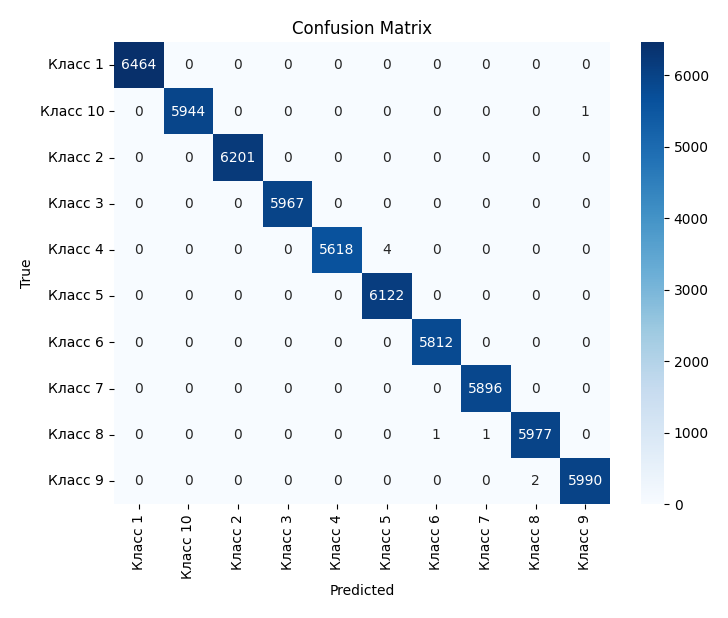
\includegraphics[scale=0.6]{pic/confusion_matrix.png}
        \caption{Матрица ошибок}
        \label{ris:confusion-matrix}
    \end{figure}
\end{center}
\vspace{1.5em}

Результаты рассчитанных метрик для реализованных моделей представлены в таблице~\ref{tabular:tableСomparison}.

\begin{table}[H]
    \onehalfspacing \caption{Метрики алгоритмов}
    \medskip
        \begin{tabular}{|l|c|c|c|}
        \hline
            \backslashbox{}{}  & precision & recall & F-score \\ \hline
            Random Forest & 0.999850046 & 0.999850000 & 0.999849998 \\  \hline 
            Gradient Boosting & 0.99998995 & 0.99959719 & 0.99979353 \\  \hline 
        \end{tabular}
    \label{tabular:tableСomparison}
\end{table}
